\documentclass[12pt,a4paper]{article}
\pagestyle{plain}
\usepackage{fullpage}
\usepackage[english]{babel}
\usepackage{enumerate}

%equations
\usepackage[fleqn]{amsmath}
\numberwithin{equation}{section}

%figures
\usepackage[dvips]{graphicx}
\graphicspath{{./images/}}
\numberwithin{figure}{section}

%excercises
\newcounter{Exercise}
\setcounter{Exercise}{1}
\usepackage[dvipsnames]{xcolor}
\usepackage{framed}
\definecolor{shadecolor}{gray}{0.9}
\usepackage{caption}

%tables
\numberwithin{table}{section}

%specials
\usepackage{textcomp} %special (greek) characters as text
%\usepackage{pstricks} %
%\usepackage{ifthen} %
%\usepackage{calc} %
%\usepackage{isotope}
\usepackage{hyperref}
\usepackage[bottom]{footmisc} %footnote below figure
\usepackage{footnpag}%number footnotes per page


%document details
\author{Koos Kortland \\ translated and adapted by K. Schadenberg}
\date{}
\title{HiSPARC Detector - Detector Array}

\begin{document}
\maketitle

\section{Introduction}
The HiSPARC projects combines a large number of detector stations (more than a hundred as of 2013) to form a network. Most of these detector stations are placed on or near schools. In this module we will take a look at how we would design an ideal network.

\section{Design Parameters}
Designing a detector and detector network works along the same lines as designing any other `product'. Every stakeholder (persons or entities with a certain interest) has a list of demands and wishes, which results in a number of design specifications or parameters which the product must meet. One important aspect in any design is the cost. Other important demands for the HiSPARC detectors were the ease of use and need for maintenance.

Of course this list specifications is not the starting point of the design process. It is the results of an (extensive) analysis of the problem. The `problem' which the HiSPARC `product' must solve is the determination of the energy and direction of primary cosmic rays. For this the arrival times and particle densities of air showers need to be measured with a certain degree of certainty (see the other modules in the series `HiSPARC Detector' and `Primary Particle' for more details).

The design of a single detector station is fixed and cannot be altered for the following assignments. We will only look at the number of placement of the stations inside our network.

\section{Station Spacing}
\begin{shaded}
\textbf{Exercise \theExercise \stepcounter{Exercise}} : List the minimal requirements of the number and placement of detectors inside our network to reconstruct the energy and direction of a high energetic cosmic ray.

In other words: How many detector stations are needed to determine the direction of the air shower and energy of the cosmic ray? How many stations are needed to determine the rays energy? Where do we need to place these detectors? Can we place them side by side or is there a certain minimum distance? Is there a maximum distance beyond which are detectors do not work?\end{shaded}

It is not easy answering the questions above without a bit more information. Figure~\ref{fig:dist_coin} shows the connection between the number of coincidences of two detector stations as a function of the distance between the stations.

\begin{figure}\begin{center}
\includegraphics[scale=0.5]{dist_coin.eps}
\caption{The average number of coincidences from a single air shower (vertical) in two detector stations as function of the distance between the two stations (horizontal). The graph shows both expected and measured numbers for HiSPARC detectors.\protect\footnotemark }\label{fig:dist_coin}
\end{center}\end{figure}
\footnotetext{HiSPARC began a little bit smaller as the NAHSA project (Nijmegen Area High School Array) located only in Nijmegen.}

\begin{shaded}
\textbf{Exercise \theExercise \stepcounter{Exercise}} : Using figure~\ref{fig:dist_coin}, what is a reasonable distance between two detector stations? \end{shaded}

\begin{shaded}
\textbf{Exercise \theExercise \stepcounter{Exercise}} : In the module `Air showers' we looked at the number of high energy cosmic rays hitting the Earth and the size of the showers (particle density away from the main shower axis) they create. Did you take this information into account when answering the previous question? If not correct your previous answer.
\end{shaded}

\section{Detector Locations}
The main focus of the HiSPARC project is on (ultra) high energetic cosmic rays.  A distance of 500~m seems a very reasonable detector spacing. Placing the detectors closer together allows us to more accurately determine the particle density distribution (and therefore primary energy) but fewer high energetic showers will be measured. The total number of multiple coincidences will be higher, but this is because more low energetic showers will be detected by more than one station at the same time.

\begin{shaded}
\textbf{Exercise \theExercise \stepcounter{Exercise}} : Use the distance between two stations mentioned above, 500~m, to spot suitable locations for HiSPARC detectors around the University of Bristol and your own school.
\begin{enumerate}[-]
\item Use (digital) maps or satellite images to search for schools and identify the ones with suitable distances between them.
\item Can you think of other locations than schools?
\item Besides distance, can you think of other criteria to select suitable locations.
\end{enumerate}
Write a well argued research proposal for a HiSPARC detector network around your own school or an extension of the existing network around the University of Bristol. Be sure to mention the coordinates of suitable detector locations and the distances between them. 
\end{shaded}

\end{document}

